\documentclass[11pt]{article}

\usepackage{fullpage}
\usepackage{hyperref}
\usepackage{amssymb}
\usepackage{amsmath}
\usepackage{amsfonts}
\usepackage{amsthm}

\usepackage{graphicx}
\graphicspath{{./figures/}}  % Path to figures folder

%%% Rob's math commands
\newcommand{\R}{\mathbb{R}} % Reals
\newcommand{\N}{\mathbb{N}} % Naturals
\newcommand{\Prob}[1]{\mathbb{P}\left[ #1\right] } % Naturals
\newcommand{\diag}[1]{\mathbf{diag}\left( #1\right)}
\newcommand{\mI}{{\bf I}}
\usepackage{mathtools}
\usepackage{mdframed} 
\usepackage{thmtools}
\newcommand{\mM}{{\bf M}}
\newcommand{\ones}{{\bf 1}}
\newcommand{\dotprod}[1]{\left< #1\right>} % product
\newcommand{\norm}[1]{ \left\| #1 \right\|}      % norm 
\DeclareMathOperator*{\argmax}{arg\,max}
\DeclareMathOperator*{\argmin}{arg\,min}
%% Packages for shaded lemmas and theorems because Robert likes these
\definecolor{shadecolor}{gray}{0.90}
\declaretheoremstyle[
headfont=\normalfont\bfseries,
notefont=\mdseries, notebraces={(}{)},
bodyfont=\normalfont,
postheadspace=0.5em,
spaceabove=1pt,
mdframed={
  skipabove=8pt,
  skipbelow=8pt,
  hidealllines=true,
  backgroundcolor={shadecolor},
  innerleftmargin=4pt,
  innerrightmargin=4pt}
]{shaded}


\declaretheorem[style=shaded,within=section]{definition}
\declaretheorem[style=shaded,sibling=definition]{theorem}
\declaretheorem[style=shaded,sibling=definition]{proposition}
\declaretheorem[style=shaded,sibling=definition]{assumption}
\declaretheorem[style=shaded,sibling=definition]{corollary}
\declaretheorem[style=shaded,sibling=definition]{conjecture}
\declaretheorem[style=shaded,sibling=definition]{lemma}
\declaretheorem[style=shaded,sibling=definition]{remark}
\declaretheorem[style=shaded,sibling=definition]{example}


\title{Alignment-free relative abundance with $K$-mers}
\author{Bob Carpenter}
\date{\today}

\usepackage[colorinlistoftodos,bordercolor=orange,backgroundcolor=orange!20,linecolor=orange,textsize=scriptsize]{todonotes}
\newcommand{\rob}[1]{\todo[inline]{\textbf{Robert: }#1}}
\newcommand{\guillaume}[1]{\todo[inline]{\textbf{Guillaume: }#1}}
\newcommand{\aaron}[1]{\todo[inline]{\textbf{Felix: }#1}}

\begin{document}

\maketitle

\abstract{\noindent Given RNA-seq data and a reference transcriptome,
  we provide a statistical model of relative abundance of transcripts
  without the need to align the reads to the transcriptome by reducing
  the reads and reference transcripts to $K$-mers.}


\begin{figure}
\centering
%\includegraphics[width=6cm]{transcipt-picture}
\caption{Example of taking a transciptone, sampling a read, and breaking into $4$-mers and the resulting frequency matrix. \rob{Not a read, a subsequence of length $L$. Furthermore, need to take all subsequences of length $L$}}
\label{fig:transcipt-picture}
\end{figure}


\rob{Questions}
\begin{enumerate}
 \item What will be our baseline of how ``well'' our method works? Compare it to the alignment method? Is there some convenient python code for this? $\norm{}$
\item  To compare the two approaches of using simplex constraint or softmax, how can we determine which one works best? Shouldn't we be comparing against a larger reference transcriptome? Or do we subsample?
\item Have we talked to the genomics group at flatiron?
\end{enumerate}

\rob{TODO}
\begin{enumerate}
\item Leave soft-max parametrization for later. Re-organize draft around just $\theta $ as a simplex variable. After all, using soft-max is just one possible  implementation, even after assuming $y$ follows a multinomial.
\end{enumerate}
\section{Introduction}

%\rob{I'm confusing terminology around transcriptome, sequence isoforms and reads. Do we have multiple transciptomes or one transciptome? By reference transciptome, is that the same thing as the isoforms?  }
We develop a fast and principled approach to determining the proportion of expressed isoforms, from a reference transciptome, using  RNA-seq data. This in turn can be used to infer what genes are being expressed by the sampled RNA-seq. This task is normally accomplished by aligning reads from the RNA-seq data to the reference transciptome. But this alignment process is computationally intensive and has other issues? 

Here we explore an approach that completely bypasses the need for aligning reads to the transciptome. Instead, we take  reads from a given RNA-seq data and break them into short $K$-mers, that is sequences of length $K$ where $K$ is of the order of $10$ to $15.$ See Figure~\ref{fig:transcipt-picture} for an illustration on a single read. 
Using a model of the process that transforms isoforms into reads, and then into $K$-mers, we are able to determine what is the most \emph{likely} set of reads and thus transciptomes that generated this set of $K$-mers.  

To give some more detail, let
 $$\Delta^p:= \{  x \in \mathbb{R}^p \; : \; \sum_{j=1}^p x_j =1, \mbox{ and }  x_i \geq 0, \quad \mbox{for } i=1,\ldots, p\}$$
 be the $p$-dimensional simplex. Assume we have a set of $G \in \mathbb{N}$ reference transcipts and a positive vector  $\theta \in \Delta^G$ where $\theta_j$  encodes the proportion of samples of the $j$th transcipts present in our data with respect to the total number of transcipts.  Reads are then taken from the transcipts, typically using RNA-seq technology, which are then shredded into $K$-mers.  There are a total of $4^K$ possible $K$-mers since there are four bases for DNA $(A, G, C, T)$. As such we can assign a number between $1$ and $4^K$ to each of  $K$-mers. 
 
Based on the process that transforms transcipts into $K$-mers, we will have a  matrix $X \in \mathbb{R}^{4^K \times G}$ that models the probability of getting a certain $K$-mer from a each transcipts, that is
\[ X_{k, g}  \; = \; p (\mbox{ $k$th K-mer} \; \mid \; \mbox{$g$th transciptome }).\]
%\rob{Something wrong, it can't be ratio of $K$-mers, and should instead be the expected number of the $k$th $K$-mer? Or the count of $K$-mers?}
We can then use this \emph{transciptome matrix} to map the ratio of transcipts to a ratio of $K$-mers, that is for  $\theta \in \Delta^G$ we have
\[   X :\theta \mapsto X\theta \in \Delta^K.\] 

 This establishes the \emph{forward model}, that takes the proportion of transcipts and returns the the proportion of $K$-mers. Yet what we have in practice is the proportion of $K$-mers. Thus we need to solve \emph{the inverse problem.}
 We do this by  counting the number  $K$-mers and store this count in a vector $y \in \mathbb{N}^{4^k}$.
We then assume that  $y$ follows a multinomial distribution and then determine $\theta$ by solving the maximum loglikelihood, that is we find $\theta^*$ such that
\[\theta^* \; \in \; \arg\max_{\theta \in  \Delta^G} \log p(\theta \; \mid \; X, y).\]
  Thus we are able to compute the most likely proportion of transcipts by observing the count of the $K$-mers, and building a matrix $X$ that maps from proportion of transcipts to proportion of $K$-mers.


In the following section we formalize the above informal descriptions, provide numerics.....


   \rob{Can we say something like $ X \theta  \approx \frac{y}{\mbox{sum}(y)}$? }

\section{Bases and $K$-mers}

The four \emph{DNA bases} are adenine (\texttt{A}),
cytosine (\texttt{C}), guanine (\texttt{G}), and thymine (\texttt{T}).
The set of DNA bases is
\[
  \mathbb{B} = \{ \texttt{A}, \texttt{C}, \texttt{G}, \texttt{T} \}.
\]
A \emph{$K$-mer} is an $K$-tuple of bases,
\[
  x = (x_1, \ldots, x_K),
  \ \textrm{where}
  \ x_1, \ldots, x_k \in \mathbb{B}.
\]
The set of $K$-mers is
\[
  \mathbb{B}^K
  = \{ (x_1, \ldots, x_K)
      : x_1, \ldots x_K \in \mathbb{B} \}.
\]
The set of $K$-mers of all lengths is
\[
  \mathbb{B}^* = \bigcup_{k=0}^{\infty} \mathbb{B}^k.
\]

\section{The transcriptome}

A \emph{transcriptome} is an indexed multiset of $K$-mers, each of
which may be of a different length,
\[
  T = T_{1}, \ldots, T_{G},
\]
with $T_{g, 1:K_g} \in \mathbb{B}^*$ for $g =1, \ldots, G$ and $K_g$ is the length of the $g$th transcriptome.  In data structure terms, the
transcriptome $T$ is a ragged array of bases.


\section{RNA-seq data}

Simple (unpaired) \emph{RNA-seq data}, after processing, consists of an indexed set of base
sequences, each of which is called a \emph{read},
\[
  R = R_1, \ldots, R_N, \ \textrm{where} \ R_n \in \mathbb{B}^J.
\]
Although not strictly necessary, we assume for simplicity that all of
the reads in the RNA-seq data are of the same length.

With \emph{paired-end} RNA-seq data, each read consists of two short RNA
sequences read from the same transcript with an unknown gap between
them on the transcriptome, so the data may be represented as
\[
  P = P_1, \ldots, P_N, \ \textrm{where} \ P_n \in \mathbb{B}^J \times
  \mathbb{B}^J.
\]
Again, although not strictly necessary, we assume all sequences are of
the same length to simplify notation.


\section{Shredding, indexing and counting $K$-mers}



\subsection{Indexing}
Since there are $4^K$ possible $K$-mers, we can 
define a bijection from the set of $K$-mers, $\mathbb{B}^K$, to the
g numbers, $\{ 0, 1, \ldots 4^K-1 \}$,
by treating each base as a digit in base 4 and reading the
$K$-mer as a number.  Following alphabetic order, let
\[
  \texttt{A} = 0,
  \quad \texttt{C} = 1,
  \quad \texttt{G} = 2,
  \quad \texttt{T} = 3.
\]
The resulting indexing sorts the $K$-mers into lexicographic order.
For example, with $K = 2$, the sixteen 2-mers are as follows.

\begin{center}
\begin{tabular}{ll|ll|ll|ll}
  \texttt{AA} & 0 & \texttt{CA} & 4 &   \texttt{GA} & 8 & \texttt{TA} & 12
  \\
  \texttt{AC} & 1 & \texttt{CC} & 5 &   \texttt{GC} & 9 & \texttt{TC} & 13
  \\
  \texttt{AG} & 2 & \texttt{CG} & 6 &   \texttt{GG} & 10 & \texttt{TG} & 14
  \\
  \texttt{AT} & 3 & \texttt{CT} & 7 &   \texttt{GT} & 11 & \texttt{TT} & 15
\end{tabular}
\end{center}
There are roughly one thousand 5-mers, because $4^5 = 1024$.  There are
roughly one million 10-mers and one billion 15-mers.

$K$-mer counts can be tabulated and stored very efficiently by using
this numbering to index into an array.  The complete set of 10-mer
counts from an RNA-seq experiment can be efficiently indexed and
stored in 4MB of memory using 32-bit counts (8MB with 64-bit counts).
Even smaller memory footprints may be achieved by packing smaller
integer representations; this could be beneficial if it enables the
counts to be stored in cache.  Shredding into 15-mers would take 4GB
(8GB) and clearly exceed cache capacity.  Beyond 15-mers, direct
indexing becomes prohibitive on readily available hardware, and either
a hashing scheme would be required or a lossy Bloom filter in order to
store approximate counts.  The memory used by hashing will be
proportional to the number of unique $K$-mers in the RNA-seq data.

\subsection{Shredding}
Suppose $K \leq N$.  A given  $N$-mer $x_{1:N}$ can be shredded into
a total of $(N - K + 1)$ $K$-mers by
\[
  x_{1:N} \ \mapsto \
  x_{1:K}, \ x_{2:K+1}, \ \ldots, \ x_{N-K+1:N}.
\]
For example, shredding   \texttt{AACAC}  into $2$-mers gives
\[
  \texttt{AACAC} \ \mapsto \
  \texttt{AA}, \ \texttt{AC}, \ \texttt{CA}, \ \texttt{AC}.
\]


\subsection{Counting}
A set of $K$-mers may be summarized with a function
$\textrm{count}_K:\mathbb{B}^* \rightarrow \mathbb{B}^K \rightarrow
\mathbb{N}$, where
$\textrm{count}_K(x)(y)$ is the number of times the $K$-mer
$y$ appears in the $N$-mer $x$.  Continuing the example above,
\begin{eqnarray*}
  \textrm{count}_2(\texttt{AACAC})(\texttt{AA}) & = & 1,
  \\
  \textrm{count}_2(\texttt{AACAC})(\texttt{AC}) & = & 2,
  \\
  \textrm{count}_2(\texttt{AACAC})(\texttt{CA}) & = & 1,
\end{eqnarray*}
and all other counts are zero. The function $ \textrm{count}_2(\texttt{AACAC}) $ can also be interpreted as a sparse vector in $\mathbb{N}^{4^k}$ with only three non-zeros elements in the indices that correspond to the $2$-mers \texttt{AA}, \texttt{AC} and \texttt{CA}.

A complete set of RNA-seq data $R = R_1, R_2, \ldots, R_N$ may then be summarized by its
$K$-mer counts by summing the counts of the individual reads %$R_{n, 1:J}$
\[
  \textrm{count}_K(R) = \sum_{n=1}^N \textrm{count}_K(R_n) \in \mathbb{N}^{4^k}
\]
\rob{Do we ever use the above notation?}
\rob{Note to remove the below? Of ``footnote'' it.}
Paired-end RNA-seq data can be shredded elementwise.  For
example, consider extracting 3-mers from a paired read.
\[
  \texttt{ATCAG} / \texttt{CGCGC}
  \ \mapsto \
  \texttt{ATC}, \texttt{TCA}, \texttt{CAG},
  \texttt{CGC}, \texttt{GCG}, \texttt{CGC}.
\]
Counts are defined for individual paired reads and a complete set of
RNA-seq data as above.
% \rob{I don't understand this Paired-end RNA-seq part or why it makes sense to mix $k$-mers of the two pairs.}




\section{Statistical model}
Suppose we have a transcriptome consisting of $G$ base sequences. Here we describe the statistical model which maps the proportion $\theta \in \Delta^G$ of base sequence in the transciptome to the count of $K$-mers.
%In a transcriptome consisting of $G$ base sequences, the only
%parameter is a vector $\alpha \in \mathbb{R}^G$, representing
%intercepts in a multi-logit regression.  $\theta_g$ represents the
%relative abundance of sequence $g$ in the transcriptome.
\rob{Re-write: Now we describe the statistical model which, given the proportion of }

\subsection{Transcriptome matrix}

A sequence $T_1, \ldots, T_g, \ldots, T_G$ in the transcriptome can be transformed into a
$4^K$-simplex representing the probability of observing a given
$K$-mer given a read of transcript $g$.  The entire transcriptome can
then be converted to a $(4^K \times G)$-matrix $X$, where column $g$ is the
simplex representing the probability of a $K$-mer being observed given
that the read was from transcript $T_g$.
%\rob{Example so I understand. If $T_g = AACAC$ and we consider the $2$-mers  in their lexicographic order, then count$(AACAC) = (1, 2, 0, 0, 1, 0, 0, 0, \cdots 0)$. So in this case, is $X_{:g} = \mbox{count}(AACAC)/| \mbox{count}(AACAC)| $? In other words, it's the proportion of observed $k$-mers in $T_g$? }

%\rob{A comment on how $X$ will ultimately depend on the users setup? But also, we offer some models of $X$, both in theory below, and in our code at XXX}
Next we discuss the distribution of $K$-mers, and how this depends on how the reads where generated. If the reads were generated \emph{uniformly}, we 
then offer a precise formula for the transciptome matrix $X$. Otherwise, $X$ will have to be given by the user.

%We will then be used to discuss a model of the probability of observing a given $K$-mer.

\subsubsection{Uniform read location}
%\rob{This section needs an intro. Here we give one way in the which the Transciptome matrix $X$ can be constructed. By note that $X$ will ultimately depend on the technology/sampling/user setup...etc}

When the reads are generated uniformly, that is every possible read from a given transcript is \emph{equally} likely, then we can compute the $X$ matrix.
To this end, first note that even if the reads are uniformly generated, the
distribution of $K$-mers will not be uniform because of edge effects
and because $K$-mers may appear more than once if $K$ is small.

For example, consider a transcript \texttt{ATGGCAATG} of nine bases.
If reads are size six and we select 4-mers within those reads,
the possibilities are as follows.
\begin{table}[h!]
\centering
  \begin{tabular}{l|l}
    \textit{Subsequences} & 4\textit{-mers}
    \\ \hline \hline
    \texttt{ATGGCA} & \texttt{ATGG, TGGC, GGCA}
    \\ \hline
    \texttt{\hspace{0.5em}TGGCAA} & \texttt{\hspace{3em}TGGC, GGCA, GCAA}
    \\ \hline
    \texttt{\hspace{1em}GGCAAT} & \texttt{\hspace{6em}GGCA, GCAA, CAAT}
    \\ \hline
    \texttt{\hspace{1.5em}GCAATG} & \texttt{\hspace{9em}GCAA, CAAT, AATG}
  \end{tabular}
  \caption{Transcipt \texttt{ATGGCAATG} broken uniformly into $6$-mer reads which are then shredded into $4$-mers.}
  \label{tab:reads}
\end{table}
%\rob{At this point, showing that Reads are produced in the same way $K$-mers are, is a bit confusing. I feel it needs some introduction/explanation. Are Reads always generated this way? Is it in fact important to explain the way Reads are generated?}
The distribution of $4$-mers resulting from uniformly sampling one of the above reads
is not expected to be uniform, but rather as follows.
\begin{center}
  \begin{tabular}{r|c||r|c}
    3\textit{-mer} & \textit{Proportion} & 3\textit{-mer} & \textit{Proportion}
    \\ \hline \hline
    \texttt{ATGG} & 1/12 & \texttt{GCAA} & 3/12
    \\ \hline
    \texttt{TGGC} & 2/12 & \texttt{CAAT} & 2/12
    \\ \hline
    \texttt{GGCA} & 3/12 & \texttt{AATG} & 1/12
  \end{tabular}
\end{center}

Assuming that every possible read  of length $J$ in a transcipt is equally likely, 
%each position in the transcript is equally likely to produce
%a read of size $J$,
 then $X_{1:4^K, g} \in \Delta^K$ is given by the proportion of $K$-mers given by all reads in the $g$th transcipt $T_g$, that is
% 
% is in the $4^K$-simplex, and is defined
%by composing count functions,
\begin{equation}
  X_{1:4^K, \, g} \; =\; \frac{z_g}{\textrm{sum}(z_g)}, \quad \mbox{where } z_g =  \sum_{j = 0}^{4^J - 1} \textrm{count}_J(T_g)(j) \cdot \textrm{count}_K(j)\; \in\; \mathbb{N}^{4^K},
\end{equation}
where $z_g$ is the total sum of $K$-mer simplexes from all reads in transcript $g$. The term
$\textrm{count}_K(j)$ is a sparse vector mapping $K$-mers to their
count in the $J$-mer represented by the integer $j$.  
This is then
weighted by $\textrm{count}_J(s)(j)$, which is the count of the $J$-mer $j$ in
the sequence $s$. If the reads were not uniform, then $z_g$ would need to be a  weighted sum that reflects how the reads are generated.
%\rob{What is $s$?}
%\[
%  X_{1:4^K, \, g}
%  = \frac{\textrm{count}_K\left(\textrm{count}_J(T_g)\right)}
%         {\textrm{sum}\left(\textrm{count}_K\left(\textrm{count}_J(T_g)\right)\right)},
%\]
%\rob{Serious notation issues: $\textrm{count}_J$ is currently defined as a function over an $N$-mer, where $N \geq J.$ Furthermore, for a given $N$-mer $T$ we have that  $\textrm{count}_J(T) \in \mathbb{N}^{4^J}.$  What does $\textrm{count}_K\left(\textrm{count}_J(T_g)\right)$ mean?  }
%\rob{Here I'm confused if this is in fact the definition of $X$ or a result of assuming uniformly distributed reads?}
%where the outer function $\textrm{count}_K$ is type lifted additively
%over functions as in the example.  Specifically, for a sequence $s$,
%and integers $K \leq J \leq \textrm{size}(s)$, the $4^K$-vector of
%$K$-mer counts found in uniformly distributed reads of size $J$ is
%\[
%  \textrm{count}_K(\textrm{count}_J(s))
%  = \sum_{j = 0}^{4^J - 1} \textrm{count}_J(s)(j) \cdot \textrm{count}_K(j)\; \in\; \mathbb{N}^{4^K}.
%\]
%\rob{So this gives sums together the counts of $K$-mer in $j$, pondered by the number of reads $j$ in $s$. This makes sense only if reads are produced according to Table~\ref{tab:reads}}
%\rob{Is $s$ a sequence of reads? 
%}
%In other words, the result $\textrm{count}_K(\textrm{count}_J(s))$ is a
%function from $K$-mer identifiers to their relative abundance in
%uniformly distributed $J$-gram reads over the sequence $s$. 
 

\subsubsection{Non-uniform read location}

\rob{Empthasize again that this is why $X$ should be given by a user, though we offer some templates.}
The probabilty of reads maybe non-uniform for several reasons.  Two
causes that have large impacts are hexamer (6-mer) binding and
position within the transcript.  In the first case, the probability of
reads being chosen from a transcript varies up to two orders of
mangitude or more based on the hexamer appearing in the first six
positions of the read.  Furthermore, the strength of these effects
depends on the priming protocol used.  In the second case, the
probability of a read can vary up to an order of magnitude or more
based on its relative position along the transcript.

Given the relative probabilities of reads originating at 6-mers, the
uniform transcriptome matrix may be adjusted by reweighting based on
the probability of the 6-mers.

Given a formula for relative probability along the transcript, the
transcriptome matrix may be further adjusted for positional effects.
In the end, the result is still a $(4^K \times G)$ transcriptome
matrix $X$.

Taken together, suppose we have transcript $T_g$ of size $N$, reads
of size $J$, and $p(n)$ is the probability of a read of size $J$
originating from position $n$.



\subsection{Observed data}

The observation $y$ is a sparse $4^K$-vector of $K$-mer counts
summed up over all reads . That is

$$ y =    \textrm{count}_K(\textrm{count}_J(s)) \; \in \; \mathbb{N}^{4^k}. $$
\rob{What is $s$? }
\rob{In the current notation, should it be instead
$$y  = \sum_{g=1}^G z_g =   \sum_{g=1}^G\sum_{j = 0}^{4^J - 1} \textrm{count}_J(T_g)(j) \cdot \textrm{count}_K(j) $$
}

This can be computed using....some technology thing ....
%This, together with 

\subsection{Transformed transcriptome matrix}
The transcriptome is representing as a $4^K \times G$ matrix $X$ as
described above. 

 The parameter is
% $\alpha \in \mathbb{R}^G$ is a
%$G$-vector whose values indicate the relative level of expression of
%each transcript on the log scale; 
$\theta \in \Delta^G$
that is in the  $G$-simplex where 
$\theta_g$ represent the proportion of each transcript $T_g$ in the transcriptome.

The key step is the transform of the transcript abundances,
represented by $\theta \in \Delta^G$, to $K$-mer
abundances, as represented by
$\phi = X \cdot \theta$.  Because
$\theta$ is in the $G$-simplex and the columns of $X$ are
in $\Delta^{4^K}$, the product $X \cdot \theta$ is in
$\Delta^{4^K}$---it just reweights the gene-level $K$-mer expressions
represented by the columns by the gene expressions represented by
$\theta$.
\rob{This section should be moved and merged with section 6.2, or just removed. }

\subsection{Sampling distribution}
	
Since $y \in \mathbb{N}^{4^k}$ is a vector of counts of $K$-mers, we make the natural assumption that $y$ was generated 
by a multinomial distribution with
\[
  y \sim \textrm{multinomial}(X \cdot \theta).
\]
Here we have used  $X \cdot \theta$, that is the proportion of observed $K$-mers, as the probabilities of sampling a $K$-mer.
\rob{Awkward point: $X \cdot \theta$ may have zero elements, and multinomial is only defined on probability vectors that are all non-zero. We can fix this numerically by looking only at the elements of  $X \cdot \theta$  that corespond to nonzero elements of $y$.}
%
%The sampling distribution $p(y \mid X, \alpha)$  for the observed
%$K$-mer counts $y$ given the transcriptome matrix $X$ and log odds
%expression simplex $\theta$ is defined to be multinomial,




\section{Posterior}

Given our statistical model, our goal is now to find the most likely 
parameters given $y$ and $X$. But first, we still need to enforce that $\theta$ is in the simplex. 
Here we show how to use the softmax mapping or an explicit projection method to enforce that $\theta$ is in the simplex. 

%\textrm{softmax}(\alpha))


\subsection{Softmax Parametrization}
%\rob{This is a choice of parametrization that only need when implementing and computing the max log-likelihood. So move this further down?}
%A $K$-\emph{simplex} is a $K$-vector $\theta$ of non-negative values
%such that $\textrm{sum}(\theta) = 1.$ 
 A vector $\alpha
\in \mathbb{R}^{G}$ can be mapped to the simplex using the softmax
function,
\begin{equation}\label{eq:softmax}
\textrm{softmax}(\alpha)_i :=\frac{e^\alpha_i}{\sum_{j=1}^G e^{\alpha_j}}, \quad \mbox{for }i=1,\ldots, G.
\end{equation}
or in a more abbreviated   notation
\[
  \textrm{softmax}(\alpha)
  = \frac{\exp(\alpha)}
         {\textrm{sum}(\exp(\alpha))} \in \Delta^{4^K},
\]
where $\exp(\alpha)$ is defined elementwise.   By construction,
$\textrm{softmax}(\alpha)$ is a simplex, because
$\textrm{softmax}(\alpha)_i > 0$ and
$\textrm{sum}(\textrm{softmax}(\alpha)) = 1$.

As a function from $K$-vectors to $K$-simplexes, softmax is many to
one, because adding a constant to each component of $\alpha$ leads to
the same result,

\[
  \textrm{softmax}(\alpha)
  = \textrm{softmax}(\alpha + \lambda \cdot \textbf{1}_K),
\]
where $\lambda \in \mathbb{R}$ and $\textbf{1}_K$ is $K$-vector
of ones. In other words,  softmax is  not an injective function.

We can however extend the softmax function into a one-to-one mapping  as follows.
The  softmax0 function defines a smooth, one-to-one mapping from
$\mathbb{R}^{K-1}$ to $K$-simplexes by
\[
  \textrm{softmax0}(\beta) = \textrm{softmax}([0 \ \, \beta]).
\]
That is, a zero element is appended to the front of the $(K-1)$-vector.
The $\textrm{softmax0}(\beta) =\theta$ function is one-to-one since we  now  $\theta_1 = (\textrm{sum}(\exp(\alpha))^{-1}$ and thus we have that
$$ \alpha_i = \ln\left(\frac{\theta_i}{\theta_0} \right), \quad \mbox{for }i=1,\ldots, K. $$.
Thus this fixed first element can be used to determine the inputs. 
%changes the interpretation of the elements from being only
%determined relative to each other to having their scale defined
%relative to the fixed first element.
\rob{Just double checking, we actually use the $ \textrm{softmax0} $ function in our code?}


\subsubsection{Prior}

The prior is a normal centered at the origin,
\[
  \alpha_g \sim \textrm{normal}(0, \lambda),
\]
for some scale $\lambda > 0$.  The smaller the scale $\lambda$, the
more parameter estimates for $\alpha_g$ are shrunk toward zero, and
thus the less relative difference in expression is allowed.

If we intend to get true zero estimates for some genes with a
continuous prior, we will need to make penalized maximum likelihood
estimates with an L1-type penalty.  Keeping to sampling notation, this
is represented by a double-exponential exponential (aka Laplace)
distribution,
\[
  \alpha_g \sim \textrm{double-exponential}(0, \lambda).
\]


\subsubsection{Posterior}

With the softmax mapping and the prior, we can now determine the most likely 
$\alpha \in \mathbb{R}^{G}$ given $y$ and $X$. That is, we now want to solve
\begin{equation}
\alpha^* \; \in \; \arg \max \log p(\alpha \; \mid \; X,y).
\end{equation}

Fortunately, this posterior distribution has a simple closed form that lends itself to optimization.
 Indeed, by Bayes's rule up to an additive constant
that does not depend on the parameters $\alpha$ we have that
\begin{align}\nonumber
  \log p(\alpha \mid X, y)& = \log p(y \mid X, \alpha) + \log p(\alpha) +
  \textrm{const.}  \\
  &= y^{\top} \cdot \log \left( X \cdot \textrm{softmax}(\alpha) \right)
          - \frac{1}{2 \cdot \lambda^2} \cdot \alpha^{\top} \cdot \alpha +\textrm{const.}  \label{eq:posterior} 
\end{align} 
 where the logarithm is applied elementwise over the vector $ X^{\top} \cdot \textrm{softmax}(\alpha).$ To determine the most likely parameters, we maximize the log posterior, that is
 
 \begin{equation} \label{eq:posteriormax} 
 \alpha^* \; \in \; \max_{\alpha \in \mathbb{R}^G} \; L(\alpha) :=  \sum_{i=1}^{4^K} y_i \cdot \log \left( x_i^\top \cdot \textrm{softmax}(\alpha) \right)
          - \frac{1}{2 \cdot \lambda^2} \cdot \alpha^{\top} \cdot \alpha,
 \end{equation}
where we have used $x_i := X_{:i}$ to denote the $i$th column of $X,$ and defined the objective function $L(\alpha)$ which is propotional to the posterior~\eqref{eq:posterior}.
We can solve~\eqref{eq:posteriormax} because it has an upper bound. 

\begin{lemma}
The objective function $L(\alpha)$ is lower bounded by 
\begin{equation}
L(\alpha) \geq 0.
\end{equation}
The gradient of $L(\alpha)$ is given by
\begin{equation}\label{eq:Lgrad}
\nabla_{\alpha}  L(\alpha) \; =\;  \sum_{i=1}^{4^K} y_i \left(\frac{\sigma(\alpha) \odot  x_i}{ x_i^{\top} \cdot \sigma(\alpha) } - \sigma(\alpha)\right) - \frac{1}{2 \cdot \lambda^2} \cdot \alpha
\end{equation}
where $\odot$ is the  elementwise multiplication also known as the Hadamard product.
\end{lemma}
\begin{proof}
Let $\ell_i(\alpha) := y_i \log \left( x_i^{\top} \cdot \textrm{softmax}(\alpha) \right)$ for the brevity. Consequently
\begin{equation}
L(\alpha) \; =  \;\sum_{i=1}^{4^K} \ell_i(\alpha)  - \frac{1}{2 \cdot \lambda^2} \cdot \alpha^{\top} \cdot \alpha.
\end{equation}

The function $\ell_i$ is upper bounded, since $\log$ is monotonically increasing , we have that 
$$ \ell_i(\alpha) = y_i \log \left( x_i^{\top} \cdot \sigma(\alpha) \right) \leq y_i \log \left( x_i^{\top} \cdot \frac{x_i}{\norm{x_i}}\right) = y_i \log \left( 1\right) =0.$$
Consequently
\[ L(\alpha) \leq 0 - \frac{1}{2 \cdot \lambda^2} \cdot \alpha^{\top} \cdot \alpha \leq 0.\]


The gradient of $\ell_i$ is given by
\begin{align}
    \nabla \ell_i(\alpha) & = \; y_i\frac{\nabla \sigma(\alpha) x_i}{ x_i^{\top} \sigma(\alpha) } \nonumber \\
          & =  y_i\frac{\sigma(\alpha) \odot  x_i -\sigma(\alpha) \sigma(\alpha)^\top x_i}{ x_i^{\top} \cdot \sigma(\alpha) }
          & \mbox{Using~\eqref{eq:siggrad}} \nonumber  \\
          & = y_i \frac{\sigma(\alpha) \odot  x_i}{ x_i^{\top} \cdot \sigma(\alpha) } - y_i\sigma(\alpha), \label{eq:ligrad}
\end{align}
where $v\odot w = \sum_{i} v_i w_i e_i$ is the hadamard product. Consequently the gradient of $L(\alpha)$ can is given by~\eqref{eq:Lgrad}.

\end{proof}

Unfortunately this function~\eqref{eq:posterior} if typically non-concave and non-convex, when the prior constant $\lambda$ is large. To illustrate, and demonstrate this, we have created a simple example in Figure~\ref{fig:nonconvex}. Fortunately, by setting the prior constant $\lambda$ sufficiently small, we have that $L(\alpha)$ is concave, as we prove in the following lemma.

\begin{figure}
\centering
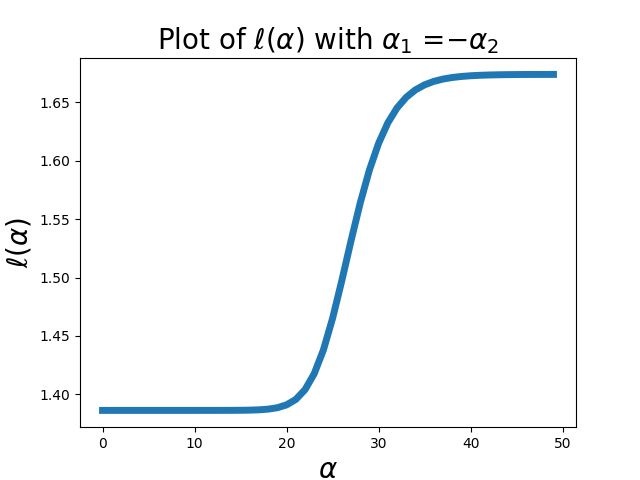
\includegraphics[width=5cm]{./figures/slice_ell} \hspace{1cm} 
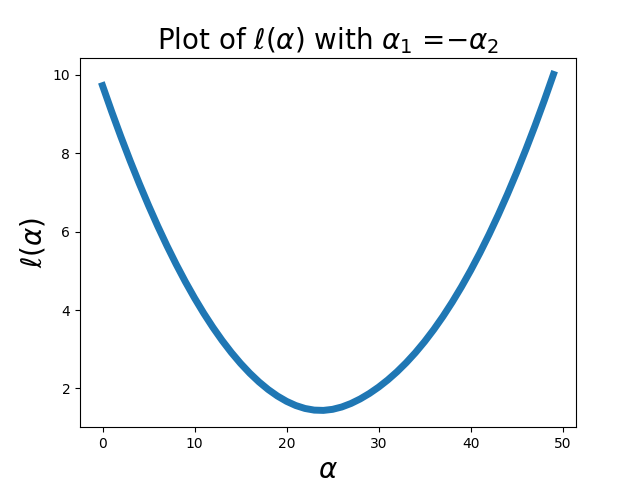
\includegraphics[width=5cm]{./figures/slice_ell_reg}
\caption{Plot of the posterior~\eqref{eq:posterior} in $\alpha$ where
$ X~=~\begin{bmatrix}
0.25 & 0.5 \\
0.75 & 0.5
\end{bmatrix}
$ and $y = [1 , 1]$, where we have plotted along the line given by $\alpha_1 = - \alpha_2$ and Left: where $\lambda = 100$ and Right: $\lambda =\sqrt{3}$.
\rob{These figures should be flipped on the $y$-axis because these as the negative log-likelihoods.}
}
\label{fig:nonconvex}
\end{figure}

\begin{lemma}
It follows that 
\begin{equation}\label{eq:Lhess}
-\left(\frac{1}{\lambda^2}-\frac{ \mbox{sum}(y)}{2}\right)  \mI  \; \preceq \; \nabla^2 L(\alpha) \; \preceq \; \left(\frac{ \mbox{sum}(y)}{2}-\frac{1}{\lambda^2} \right) \mI
\end{equation}
Consequently if $\lambda \leq \sqrt{\tfrac{2}{ \mbox{sum}(y)}}$ then $L(y)$ is a concave function.
\end{lemma}
\begin{proof}
Taking the derivative again in~\eqref{eq:ligrad} we have that
\begin{align}
\nabla^2 \ell_i(\alpha) & =   y_i \left(\frac{\nabla \sigma(\alpha)  \diag{ x_i}}{ x_i^{\top} \cdot \sigma(\alpha) } - \frac{ (\nabla \sigma(\alpha) x_i)(\sigma(\alpha)  \odot x_i)^\top}{( x_i^{\top} \cdot \sigma(\alpha) )^2}  \right) -y_i\nabla \sigma(\alpha). \label{eq:tempsoinjz4}
\end{align}
    Next note that 
    \begin{align*}
        \frac{ (\nabla \sigma(\alpha) x_i)(\sigma(\alpha)  \odot x_i)^\top}{( x_i^{\top} \cdot \sigma(\alpha) )^2} & = \frac{ (\sigma(\alpha) \odot x_i - \sigma(\alpha)  \sigma(\alpha) ^\top x_i )(\sigma(\alpha)  \odot x_i)^\top}{( x_i^{\top} \cdot \sigma(\alpha) )^2} \\
        &= \frac{ (\sigma(\alpha) \odot x_i) (\sigma(\alpha) \odot x_i)^\top  }{( x_i^{\top} \cdot \sigma(\alpha) )^2} - \frac{\sigma(\alpha) (\sigma(\alpha) \odot x_i)^\top } { x_i^{\top} \cdot \sigma(\alpha) }
    \end{align*}

Furthermore
\begin{align*}
    \frac{\nabla \sigma(\alpha)  \diag{ x_i}}{ x_i^{\top} \cdot \sigma(\alpha) } & = \frac{  \diag{\sigma(\alpha)\odot x_i}}{ x_i^{\top} \cdot \sigma(\alpha) } -\frac{\sigma(\alpha) (\sigma(\alpha) \odot x_i)^\top }{ x_i^{\top} \cdot \sigma(\alpha) }
\end{align*}
Inserting the above two identities into~\eqref{eq:tempsoinjz4}, using~\eqref{eq:siggrad} and after some cancellation gives the resulting identity
\begin{align}
\nabla^2 \ell_i(\alpha)& = y_i \left(\frac{  \diag{\sigma(\alpha)\odot x_i}  }{ x_i^{\top} \cdot \sigma(\alpha) } -\frac{ (\sigma(\alpha) \odot x_i) (\sigma(\alpha) \odot x_i)^\top  }{( x_i^{\top} \cdot \sigma(\alpha) )^2}  +\sigma(\alpha)\sigma(\alpha)^\top - \diag{\sigma(\alpha)}\right). \label{eq:tempsoinjz4}
\end{align}

To temporarily simplify our notation, let
\[v_i := \frac{\sigma(\alpha) \odot x_i}{x_i^{\top} \cdot \sigma(\alpha)}\]
and note that $(v_i)_j \geq 0$ since $(\sigma(\alpha) \odot x_i)_j \geq 0$ and furthermore 
\[\sum_{j} (v_i)_j = \sum_{j=1}^n \frac{\sigma(\alpha)_j (x_i)_j}{x_i^{\top} \cdot \sigma(\alpha)} =\frac{x_i^{\top} \cdot \sigma(\alpha)}{x_i^{\top} \cdot \sigma(\alpha)} =1. \]
Thus $v_i$ is a probability vector. Using this notation we have that
\begin{align}
\nabla^2 \ell_i(\alpha)& = y_i \left( \diag{v_i} - v_iv_i^\top +\sigma(\alpha)\sigma(\alpha)^\top - \diag{\sigma(\alpha)} \right). \label{eq:tempsoinjz4}
\end{align}

Let  $\mM = v_iv_i^\top -\diag{v_i} +\diag{\sigma(\alpha)} -\sigma(\alpha)\sigma(\alpha)^\top$. By applying Lemma~\ref{lem:probmat} twice we have that $- \frac{1}{2}\mI \preceq \mM \preceq \frac{1}{2}\mI$, which shows that
\begin{align}
-\frac{y_i}{2}\mI \preceq \; \nabla^2 \ell_i(\alpha)& \preceq  \frac{y_i}{2}\mI
\end{align}
The proof of~\eqref{eq:Lhess} now follow by summing up over the above and using that $\nabla^2 \frac{1}{2 \lambda^2}\alpha^\top \alpha = \frac{1}{\lambda^2} \mI.$
\end{proof}


%\subsubsection{Posterior gradient}

\rob{**previous version***}
We can also efficiently compute the gradient\footnote{The derivative is easy to work out
  by passing \url{matrixcalculus.org} the query
  \begin{center}\texttt{y' * log
(X * exp(a) / sum(exp(a))) - a' * a / (2 * lambda)}\end{center}
and then simplifying using $\textrm{softmax}$.} of posterior using 
%Efficient maximum penalized likelihood estimation and full Bayesian inference
%require evaluating gradients of the posterior with respect to the parameters
%$\alpha$.  The gradient is
%%
\begin{align}
  \nabla\!_{\alpha} \, \log p(\alpha \mid X, y) + \log p(\alpha)
& = \
    t \odot \textrm{softmax}(\alpha)
    - \textrm{softmax}(\alpha)^{\top}\! \cdot t \cdot \textrm{softmax}(\alpha)
    - \frac{\displaystyle \alpha}{\displaystyle \lambda} \nonumber\\
    &= t \odot \textrm{softmax}(\alpha)
    - \mbox{sum}(y)\cdot \textrm{softmax}(\alpha)
    - \frac{\displaystyle \alpha}{\displaystyle \lambda}
\end{align}
where
\[
  t = X^{\top}\! \cdot (y \oslash (X \cdot \textrm{softmax}(\alpha)))
\]
and $\odot$ represents elementwise multiplication and $\oslash$
elementwise division. To arrive at the simplification we made to get the second equality we used that
$$  t = X^{\top}\! \cdot (y \oslash (X \cdot \textrm{softmax}(\alpha))) =  X^{\top}\! \cdot \diag{X \cdot \textrm{softmax}(\alpha)}^{-1}  y$$
and thus
\begin{align*}
  \textrm{softmax}(\alpha)^{\top}\! \cdot t \cdot \textrm{softmax}(\alpha) & = 
 \textrm{softmax}(\alpha)^{\top}\! \cdot X^{\top}\! \cdot \diag{X \cdot \textrm{softmax}(\alpha)}^{-1}  y \cdot \textrm{softmax}(\alpha) \\
&= (X  \textrm{softmax}(\alpha))^{\top} \cdot \diag{X \cdot \textrm{softmax}(\alpha)}^{-1}  y \cdot \textrm{softmax}(\alpha) \\
& = \ones ^\top  y \cdot \textrm{softmax}(\alpha)
 = \mbox{sum}(y)\cdot \textrm{softmax}(\alpha),
\end{align*}
 where we used that $v^\top \diag{v}^{-1} = \ones^\top$. 


\subsection{Simplex Constraint}

Instead of maximizing~\eqref{eq:posterior} using the softmax parametrization, we can instead impose the simplex as a constraint and solve
\begin{align}
\theta^* \; \in \; \arg \max_{\theta \in \Delta^G}  \log p(\theta \mid X, y) &= y^{\top} \cdot \log \left( X \cdot \theta \right)
         +\log p(\theta)+\textrm{const.} \label{eq:posterior-const}
\end{align} 
As for the prior $p(\theta)$, since $\theta$ is in the simplex, we now choose a symmetric Dirchlet  prior over the parameters where
\begin{equation}
p(\theta) \; = \; \frac{\Gamma(\beta G)}{\Gamma(\beta)^G} \prod_{i=1}^G \theta_i^{\beta -1}, 
%\quad \mbox{where}\quad B(\beta) = \frac{\prod_{i=1}^G \Gamma(\beta_i)}{\Gamma(\sum_{i=1}^G \beta_i)}
\end{equation}
where $\beta>0$ and $\Gamma$ is the gamma function $\Gamma(z) : = \int_{0}^{\infty} x^{z-1}e^{-x}dx.$
Consequently~\eqref{eq:posterior-const} is equivalent to solving
 \begin{align}
\theta^* \; \in \; \arg \max_{\theta \in \Delta^G}   y^{\top} \cdot \log \left( X \cdot \theta \right)
         +(\beta-1)\sum_{i=1}^G\log\theta_i =: f(\theta). \label{eq:posterior-const}
\end{align} 

% \begin{align}
%\theta^* \; \in \; \arg \max_{\theta \in \Delta^d}   \sum_{i=1} y_i \cdot \log \left( x_i^\top \theta \right)
%         +(\beta-1)\sum_{i=1}^n\log\theta_i. \label{eq:posterior-const}
%\end{align} 


For the above function $f(\theta)$ we have that
\begin{align}
\nabla f(\theta) &= \sum_{j=1}^n \frac{y_j x_j}{x_j^\top \theta} + (\beta-1 ) \diag{\theta}^{-1} \ones\\
&= X^\top y \;\diag{X  \cdot\theta}^{-1}+ (\beta-1 ) \diag{\theta}^{-1} \ones
\end{align}
We can solve~\eqref{eq:posterior-const} iteratively using the Exponentiated Gradient Descent (EGA) method. At each iteration, EGA minimizes a linearization of the objective together with KL divergence, that is
\begin{align}\label{eq:EGA}
\theta^{t+1} & = \argmin_{\theta} -f(\theta^t) - \nabla f(\theta^t)^\top(\theta -\theta^t) + \frac{1}{\gamma_t} KL(\theta,\theta^t),
\end{align}
where $\gamma_t >0$ is a step length and $ KL(p,q) = \sum_i p_i \log\left(\frac{p_i}{q_i} \right)- \sum_i(p_i-q_i)$. Fortunately~\eqref{eq:EGA} has a closed form solution given by
\begin{align}\label{eq:EGAupdate}
\theta^{t+1} &=  \frac{\theta^t_i \exp( \gamma_t  \nabla_{i}f(\theta^t) )}{\sum_{j=1}^G\theta^t_j \exp( \gamma_t  \nabla_{j}f(\theta^t) ) }.
\end{align}
Note that at every iteration we have that $\theta^t \in \Delta^G.$ The $\gamma_t$ are the step size, for which we use

\begin{equation}
\gamma_t \; := \; \frac{\sqrt{2}}{\norm{\nabla f(\theta^t) }_{\infty} \sqrt{t+1}}
\end{equation}

\rob{Relative smoothness lower bound}
\[ y\log(x) \geq^? y \log(w) + y\frac{x-w}{w} + L \cdot KL(x,w)\]
Re-arranging
\[y \log \left(\frac{x}{w}\right)-y\frac{x}{w} +y \geq   L \cdot \left( x\log\left(\frac{x}{w}\right)-x+w \right)\]

\subsubsection{Relative smoothness}

Consider the density of the multinomial distribution
\begin{equation}\label{eq:multi}
p(x \; \mid \; \pi, N)\; = \;\frac{N!}{x_1! \ldots x_n!} \prod_{i=1}^n \pi_i^{x_i} \;= \;h(x) e^{\sum_{i=1}^n x_i \log(\pi_i)}
\end{equation}
where $\sum_{i=1}^n x_i = N$ and $h(x) =  \frac{n!}{x_1! \ldots x_n!} .$ In terms of the exponential family we have that the canonical parameters are $\eta = (\log(\pi_1), \ldots, \log(\pi_n))$, the sufficient statistics $S(x) = x$, the partition function $A(\eta)=0$. In the natural parameters we have that
\[ p(x \; \mid \; \eta) \; =\; h(x) e^{ x^\top \eta}. \]

Taking the derivative in $\eta$ of the log-likelihood is given by
\[\nabla_{\eta}\log p(x \; \mid \; \eta)=  x. \]


Alternatively, if we use that $\pi \in \Delta^n $ and $\sum_{i=1}^n x_i = N$ we can write $\pi_n = 1 - \sum_{j=1}^{n-1}\pi_{j}$ and $x_n = N- \sum_{i=1}^{n-1} x_i.$
Using this  we have that~\eqref{eq:multi} is given by
\begin{align}
\label{eq:multisub}
p(x \; \mid \; \pi) & = \frac{n!}{x_1! \ldots x_n!} (1 - \sum_{j=1}^{n-1}\pi_{j})^{N- \sum_{i=1}^{n-1} x_i} \prod_{i=1}^{n-1} \pi_i^{x_i} \nonumber \\
&= \; h(x) (1 - \sum_{j=1}^{n-1}\pi_{j})^{N} \prod_{i=1}^{n-1} \left(\frac{\pi_i}{(1 - \sum_{j=1}^{n-1}\pi_{j})}\right)^{x_i} \nonumber \\
& =\;h(x) e^{\sum_{i=1}^{n-1} x_i \log\left(\frac{\pi_i}{1 - \sum_{j=1}^{n-1}\pi_{j}}\right) + N\log(1 - \sum_{j=1}^{n-1}\pi_{j})} \nonumber \\
& =\;h(x) e^{\sum_{i=1}^{n-1} x_i \eta_i + A(\eta)} 
\end{align}
where
\begin{align*}
\eta_i &= \log\left(\frac{\pi_i}{1 - \sum_{j=1}^{n-1}\pi_{j}}\right), \quad \mbox{for }i=1,\ldots,n-1. \\ 
\pi_i & = \frac{e^{\eta_i}}{1+ \sum_{j=1}^{n-1}e^{\eta_{j}}}, \quad \mbox{for }i=1,\ldots,n-1. \\ 
A(\eta) &= N\log(1 - \sum_{j=1}^{n-1}\pi_{j}) \; = \; -N\log(1 + \sum_{j=1}^{n-1}e^{\eta_{j}}).
\end{align*}
This now fits the format of the exponential family. Furthermore, the $\eta$'s are only unconstrained.

Thus the log-likelihood in this case is given by
\begin{equation}
\log p(x \; \mid \; \eta)=  h(x) +x^\top \eta -N\log(1 + \sum_{j=1}^{n-1}e^{\eta_{j}}).
\end{equation}

According to Proposition 1 in~\cite{MarkEM} we have that the negative loglikelihood $L(\eta) : = -\log p(x \; \mid \; \eta)$ has a smooth lower bound given by
\begin{align*}
L(\eta) \; \leq \;  L(\eta^0) +  \dotprod{ \nabla L(\eta^0), \eta -\eta^0  } + D_A(\eta,\eta_0)
\end{align*}
where $D_A(\eta,\eta_0)$ is the divergence induced by the partition function $A(\eta)$, that is
\begin{align}
D_A(\eta,\eta_0) \; : = \; A(\eta) - A(\eta_0) - \dotprod{\nabla A(\eta_0), \eta - \eta_0}
\end{align}
Plugging in the definition of $L$ and $D_A$ we have that

\begin{align*}
-x^\top \eta -A(\eta)& \leq \; -x^\top \eta^0-A(\eta^0)-  \dotprod{ x+\nabla A(\eta^0), \eta -\eta^0  } + A(\eta) - A(\eta_0) - \dotprod{\nabla A(\eta_0), \eta - \eta_0}\\
& \implies \\
0 & \leq  A(\eta) - A(\eta_0) - \dotprod{\nabla A(\eta_0), \eta - \eta_0},
\end{align*}
which holds if $A$ is convex.

\rob{Recovering $\theta$}
So we could solve this model, and then recover $\theta$ by solving the linear system
\[X \cdot \theta = \pi.\]
This linear system is probably over-determined, so we can use the least-squares solution.


Taking the derivative in $\eta$ of the log-likelihood is given by
\[\nabla_{\eta}\log p(x \; \mid \; \eta)=  x + \nabla A(\eta) = x -\frac{1}{1 + \sum_{j=1}^{n-1}e^{\eta_{j}}} e^{\eta}. \]
Setting to zero and isolating we have that
\[ \eta = \log(x) + \log\left(1 + \sum_{j=1}^{n-1}e^{\eta_{j}}\right).\]
\rob{We could solve this nonlinear equation using regularized Newton or something? }


\rob{Is the objective relatively smooth with respect to the KL divergence? Is so, then smoothness dictates the stepsize. Read here \url{https://arxiv.org/pdf/2202.12843.pdf}. Also, didn't mark Schmidt prove already relative smooth for the log likelihood of the entire exponential family? And multinomial is a special see here \url{http://www.cs.cmu.edu/~epxing/Class/10708-16/note/10708_scribe_lecture5.pdf}}
That is
\[\nabla^2 \log(x^\top \theta) =   \]

%we could use entropy, that is $p(\theta) = -\sum_{i=1}^G \theta_i \log(\theta_i).$ But what does this mean in terms of probabilistic assumptions?
%
%The advantage of~\eqref{eq:posterior-const} is that, with a strongly convex prior, the resulting optimization problem is strongly convex and smooth, and thus can be provenly solve with L-BFGS.

\section{Estimating expression}

\rob{Are all these alternative approaches to maximizing the posterior of $\alpha$?}
\subsection{Bayesian posterior mean estimate}

The Bayesian \emph{posterior mean estimate} is the parameter's
expected value conditioned on the observed data,
\begin{eqnarray*}
  \widehat{\alpha}
  & = & \mathbb{E}\!\left[\alpha \mid X, y \, \right]
  \\[6pt]
  & = & \int_{\mathbb{R}^G} \alpha \cdot p(\alpha \mid X, y) \, \textrm{d}\alpha.
\end{eqnarray*}
The posterior mean estimate minimizes expected square estimation error
for $\alpha$ if the model is well specified.

Given a sampler that can produce Markov chain Monte Carlo (MCMC) draws
distributed according to the posterior
\[
  \alpha^{(m)} \sim p(\alpha \mid X, y),
\]
the posterior mean estimate may be calculated as
\[
  \widehat{\alpha} \approx \frac{1}{M} \sum_{m = 1}^M \alpha^{(m)}.
\]
As $M \rightarrow \infty$, the approximation converges to the true
value.  Assuming the Markov chain is geometrically ergodic, the MCMC
central limit theorem applies, providing a convergence rate of
$\mathcal{O}\left(1 / \sqrt{M}\right)$.  In practice, a few hundred
effective draws brings the expected error on $\widehat{\alpha}$ due to
MCMC down to less than a tenth of the posterior standard deviation of
$\alpha$.

\subsection{Maximum a posteriori estimate}
\rob{Why are we mentioning this?}
The \emph{max a posteriori} (MAP) estimate for $\alpha$ is given by
choosing the parameter value $\alpha^*$ that maximizes the posterior
density,
\[
  \alpha^* = \textrm{arg\,max}_{\alpha} \,
  \log \textrm{multinomial}(y \mid x \cdot \textrm{softmax}(\alpha))
  + \log \textrm{normal}(\alpha \mid 0, \lambda \cdot \textrm{I}).
\]
This is not a Bayesian estimate because it does not average over
posterior uncertainty.


\subsection{Maximum penalized likelihood estimate}

A pure frequentist estimate may be defined by casting the normal prior
on the parameters as a penalty function based on the $\textrm{L}_2$
norm,
\[
  -\frac{1}{2 \cdot \lambda^2} \cdot \alpha^{\top}\!\! \cdot \alpha.
\]

Replacing the normal prior in the definition of the MAP estimate with
the $\textrm{L}_2$ penalty defined above, the
\emph{penalized maximum likelihood estimate} (MLE) is defined as
\[
  \alpha^* = \textrm{arg\,max}_{\alpha} \,
  \log \textrm{multinomial}(y \mid x \cdot \textrm{softmax}(\alpha))
  - \frac{1}{2 \cdot \lambda^2} \cdot \alpha^{\top}\!\! \cdot \alpha.
\]


\section*{References}

\begin{itemize}
\item Biases in Illumina transcriptome sequencing caused by random
  hexamer priming Kasper D. Hansen,1,* Steven E. Brenner,2 and
  Sandrine Dudoit1,3.  Nucleic acids research.
\end{itemize}


\appendix

\section{Useful Lemmas}


\begin{lemma}
The Jacobian $\nabla \textrm{softmax}(\alpha) \in \R^{T \times T}$ of  softmax~\eqref{eq:softmax} satisfies
\begin{equation}\label{eq:siggrad}
     \nabla \textrm{softmax}(\alpha)  = \diag{\textrm{softmax}(\alpha)} -\textrm{softmax}(\alpha)\textrm{softmax}(\alpha)^\top, 
\end{equation}
where $\diag{\textrm{softmax}(\alpha)} \in \R^{T \times T}$ is a diagonal matrix. Consequently we have that
\begin{equation}\label{eq:sigmamatrxbound}
  0  \preceq \nabla \textrm{softmax}(\alpha) \preceq \frac{1}{2} \mI_T,
\end{equation}
where $\mI_T \in \R^{T \times T}$ is the identity matrix. 
\end{lemma}
\begin{proof}
Taking the derivative of~\eqref{eq:softmax} we have that
    \begin{align*}
    \nabla_{\alpha_i} \sigma (\alpha)_j &=  \frac{e^{\alpha_j} \delta_{ij}}{\sum_{j=1}^T e^{\alpha_j}} -\frac{e^{\alpha_j}e^{\alpha_i}}{(\sum_{j=1}^T e^{\alpha_j})^2}  \\
    &= \textrm{softmax}(\alpha)_j \delta_{ij} - \textrm{softmax}(\alpha)_j\textrm{softmax}(\alpha)_i
\end{align*}
    Summing up over $i,j=1,\ldots, T$ gives~\eqref{eq:siggrad}. Finally~\eqref{eq:sigmamatrxbound} follows from Lemma~\ref{lem:probmat}.
\end{proof}



\begin{lemma}\label{lem:probmat}
Let $p \in \R^n$ be a vector of probabilities with $\sum_{i=1}^n p_i =1.$ It follows that
\begin{equation}
 0  \preceq   \diag{p} - p p^\top \preceq  \frac{n}{2} \left( \frac{1}{n}\mI - \frac{1}{n^2}\ones \ones^\top  \right) = \frac{1}{2}\mI - \frac{1}{n}\ones \ones^\top \preceq  \frac{1}{2}\mI .
\end{equation}
\end{lemma}
\begin{proof}
Let $\mM =\diag{p} - p p^\top.$
Using Gershgorin's circle theorem we have that every eigenvalue of $\mM$ satisfies
\[ |\mM_{ii} - \lambda  | \leq \sum_{j\neq i} |\mM_{ij}| \]
That is
\[ |p_i(1-p_i) - \lambda  | \leq \sum_{j\neq i} p_i p_j = p_i(1-p_i). \]
Consequently
\[0 \leq \lambda \leq 2 p_i(1-p_i).\]
Thus $\mM$ is positive semi-definite. The argument for the upper bound is that $\mM(p) \preceq \mM(1/n , \ldots , 1/n)$ which follows by showing that 
\[ \left[ \frac{1}{n}, \ldots, \frac{1}{n}\right]= \arg\max_{p^*} \max_v \frac{v ^\top \mM(p) v}{v ^\top \mM(p^*) v}\]


Alternative argument. For the upper bound clearly $\mM \preceq \diag{p}.$ Consequently $\lambda_{\max}(\mM) \leq \lambda_{\max}(\diag{p}) = \max_i p_i \leq 1.$
\end{proof}
\end{document}
